\subsection{Testing}
\subsubsection{Analisi Statica - CodeMR}

\begin{figure}[H]
    \centering
    \begin{minipage}{0.45\textwidth}
        \centering
        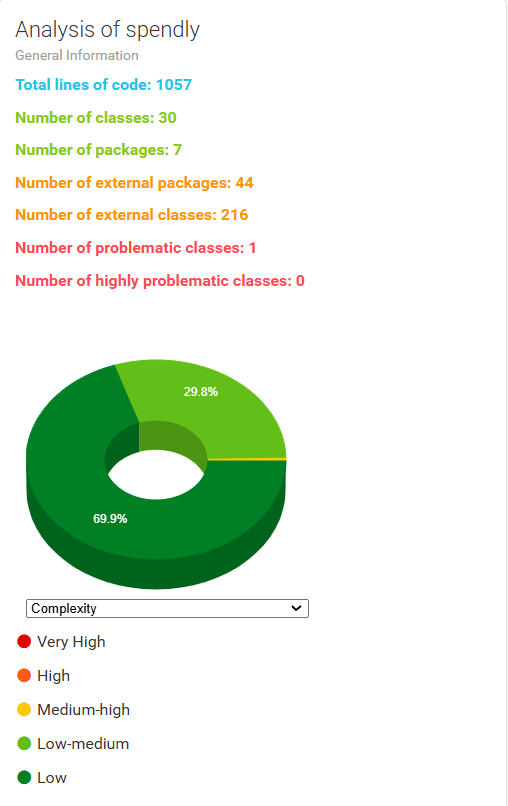
\includegraphics[width=\textwidth]{images/Complexity_iter2.png}
        \caption{Complexity}
        \label{fig:Complexity_iterazione2}
    \end{minipage}
    \hfill
    \begin{minipage}{0.45\textwidth}
        \centering
        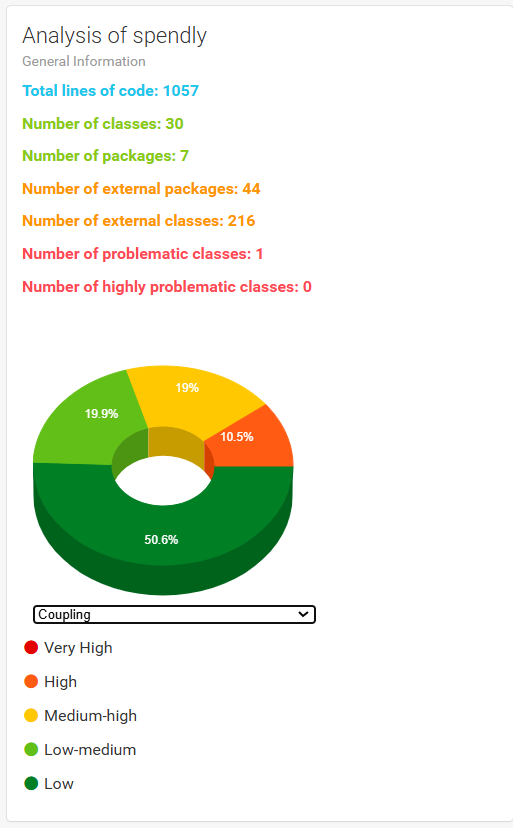
\includegraphics[width=\textwidth]{images/Coupling_iter2.png}
        \caption{Coupling}
        \label{fig:Coupling_iterazione2}
    \end{minipage}
\end{figure}

\begin{figure}[H]
    \centering
    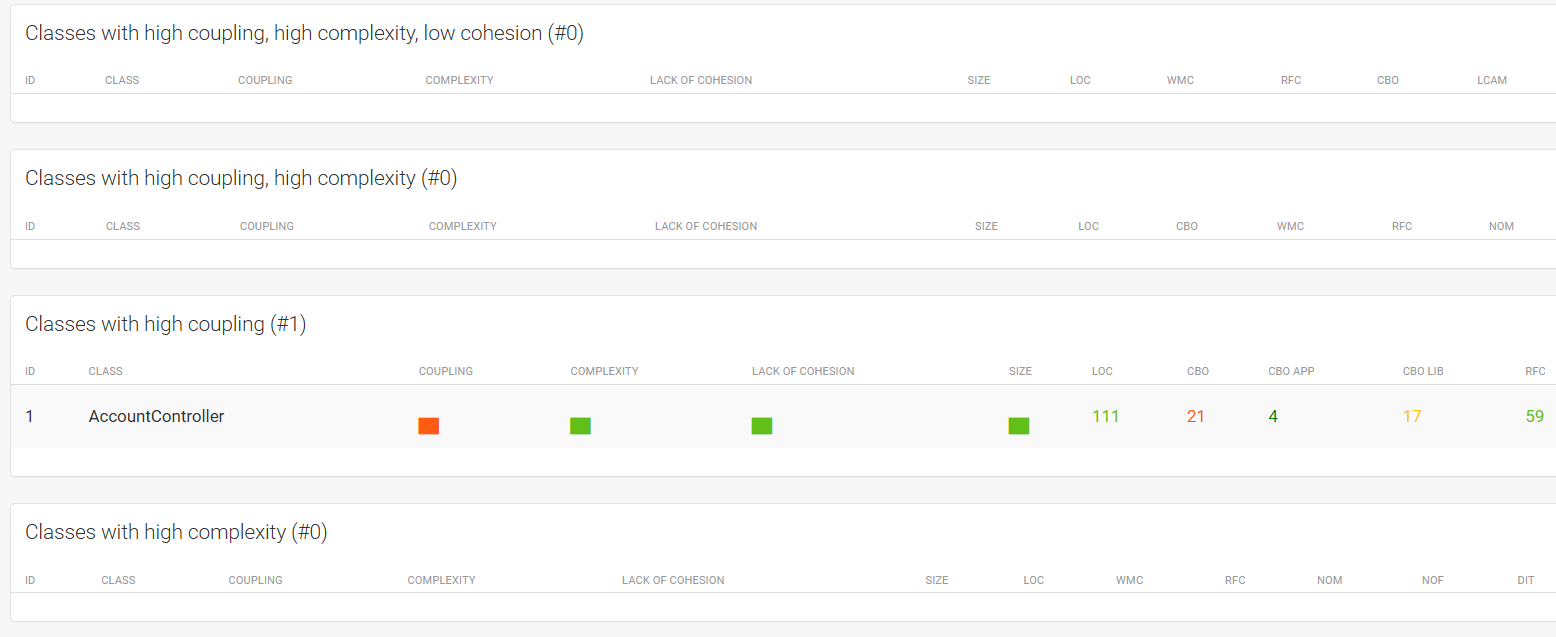
\includegraphics[width=0.9\textwidth]{images/Problem_iter2.png}
    \caption{Problemi classi}
    \label{fig:Problemi_iterazione2}
\end{figure}



\begin{figure}[H]
    \centering
    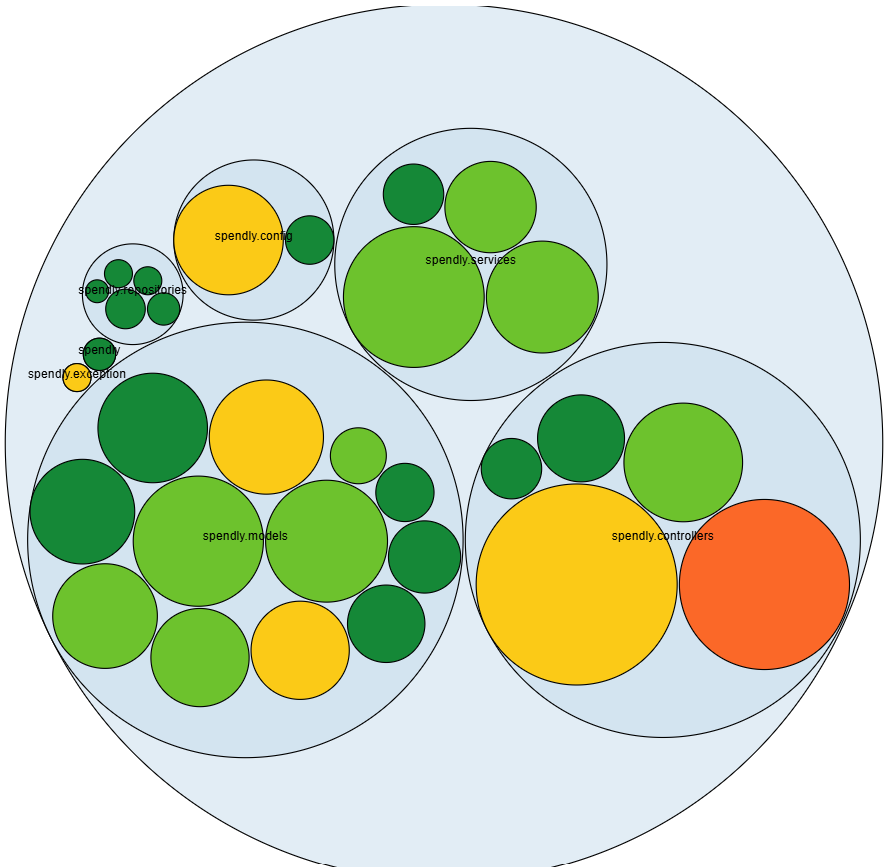
\includegraphics[width=0.6\textwidth]{images/Package_iter2.png}
    \caption{Struttura dei package}
    \label{fig:Package_iterazione2}
\end{figure}

\subsubsection{API Costi}

Questa sezione documenta le API relative alla gestione dei **costi** nel sistema **Spendly**, inclusi la creazione, l'eliminazione e la visualizzazione dei costi di utenti e gruppi. Ogni test verrà mostrato con un'**immagine dei risultati**.

\paragraph{Aggiunta di un Costo}  

\begin{itemize}
    \item \textbf{Endpoint:} \texttt{POST /api/costs?username=\{username\}}
    \item \textbf{Descrizione:} Permette all'utente autenticato di aggiungere un nuovo costo, eventualmente associandolo a un gruppo.
    \item \textbf{Parametri:}
    \begin{itemize}
        \item \texttt{importo} (double) - Importo della spesa.
        \item \texttt{tipologia} (string) - Tipo di spesa.
        \item \texttt{groupId} (integer, opzionale) - ID del gruppo a cui associare il costo.
    \end{itemize}
\end{itemize}
\newpage
\begin{figure}[h!]
    \centering
    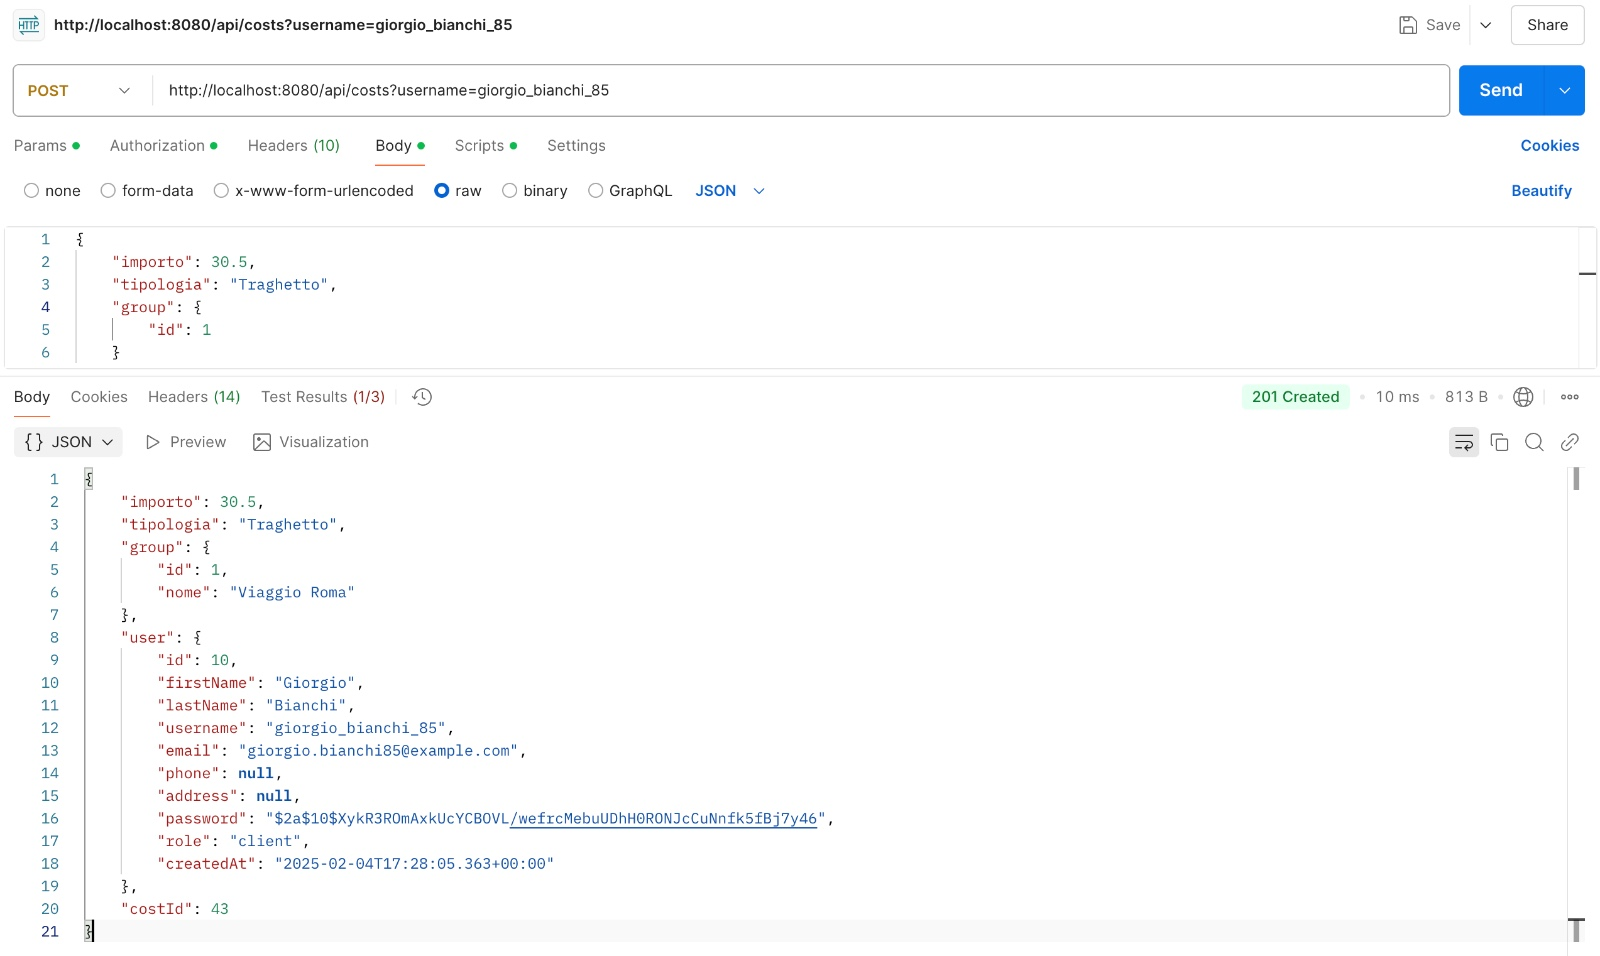
\includegraphics[width=0.9\textwidth]{images/createCost.jpeg}
    \caption{Risultato API Aggiunta Costo}
    \label{fig:api_add_cost}
\end{figure}

\paragraph{Eliminazione di un Costo}  

\begin{itemize}
    \item \textbf{Endpoint:} \texttt{DELETE /api/costs/\{costId\}}
    \item \textbf{Descrizione:} Permette all'utente autenticato di eliminare un costo precedentemente registrato.
    \item \textbf{Parametri:}
    \begin{itemize}
        \item \texttt{\{costId\}} (integer) - ID del costo da eliminare.
    \end{itemize}
\end{itemize}

\begin{figure}[h!]
    \centering
    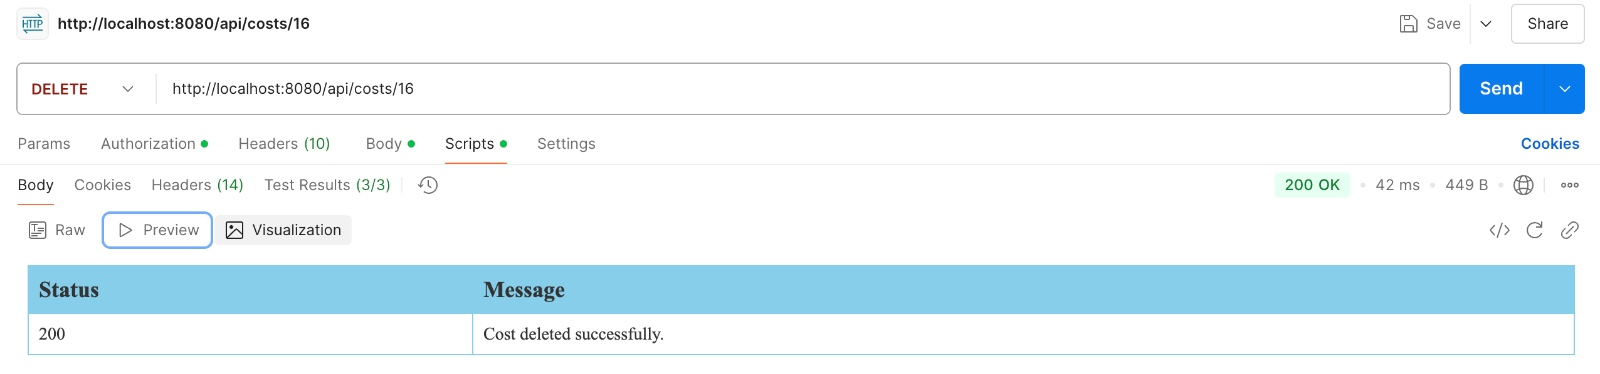
\includegraphics[width=0.9\textwidth]{images/deleteCost.jpeg}
    \caption{Risultato API Eliminazione Costo}
    \label{fig:api_delete_cost}
\end{figure}

\paragraph{Visualizzazione Costi Utente}  

\begin{itemize}
    \item \textbf{Endpoint:} \texttt{GET /api/costs?username=\{username\}}
    \item \textbf{Descrizione:} Restituisce la lista di tutti i costi registrati dall'utente autenticato.
\end{itemize}

\begin{figure}[h!]
    \centering
    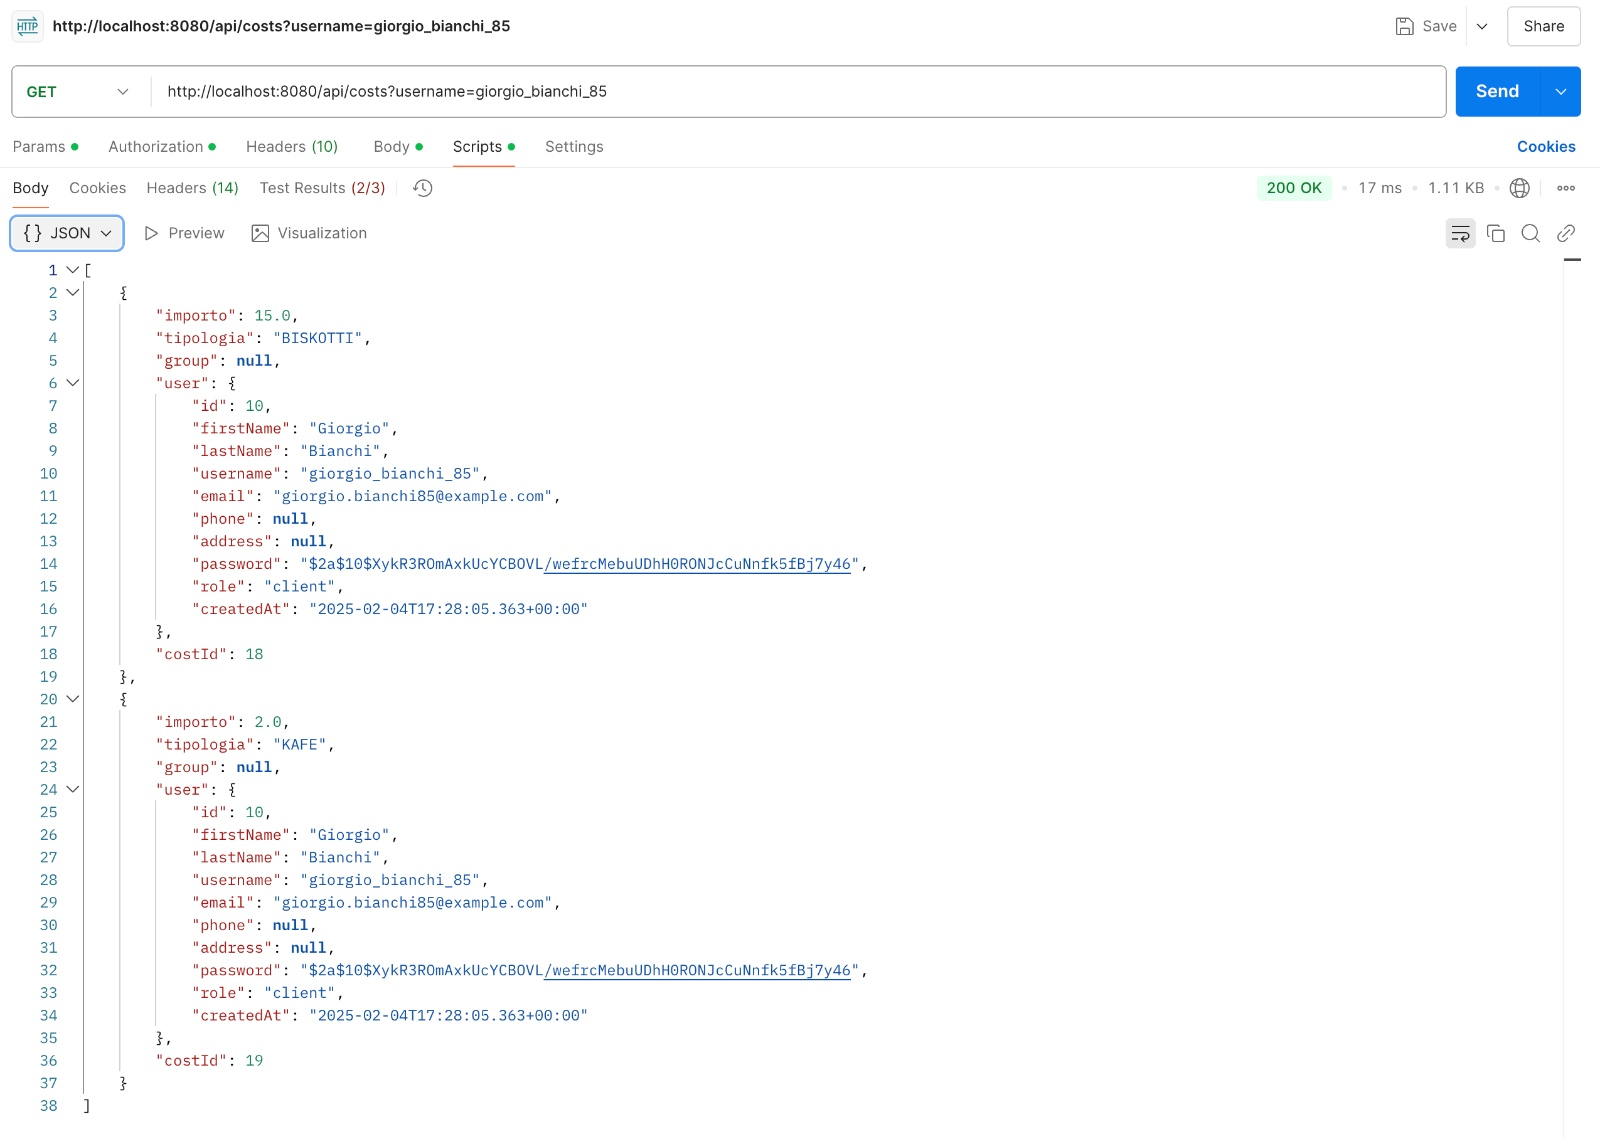
\includegraphics[width=0.9\textwidth]{images/getUserCosts.jpeg}
    \caption{Risultato API Visualizzazione Costi Utente}
    \label{fig:api_view_user_costs}
\end{figure}

\paragraph{Visualizzazione Costi di un Gruppo}  

\begin{itemize}
    \item \textbf{Endpoint:} \texttt{GET /api/costs/group/\{groupId\}}
    \item \textbf{Descrizione:} Restituisce la lista di tutti i costi associati a un gruppo, accessibile solo dai membri del gruppo.
\end{itemize}

\begin{figure}[h!]
    \centering
    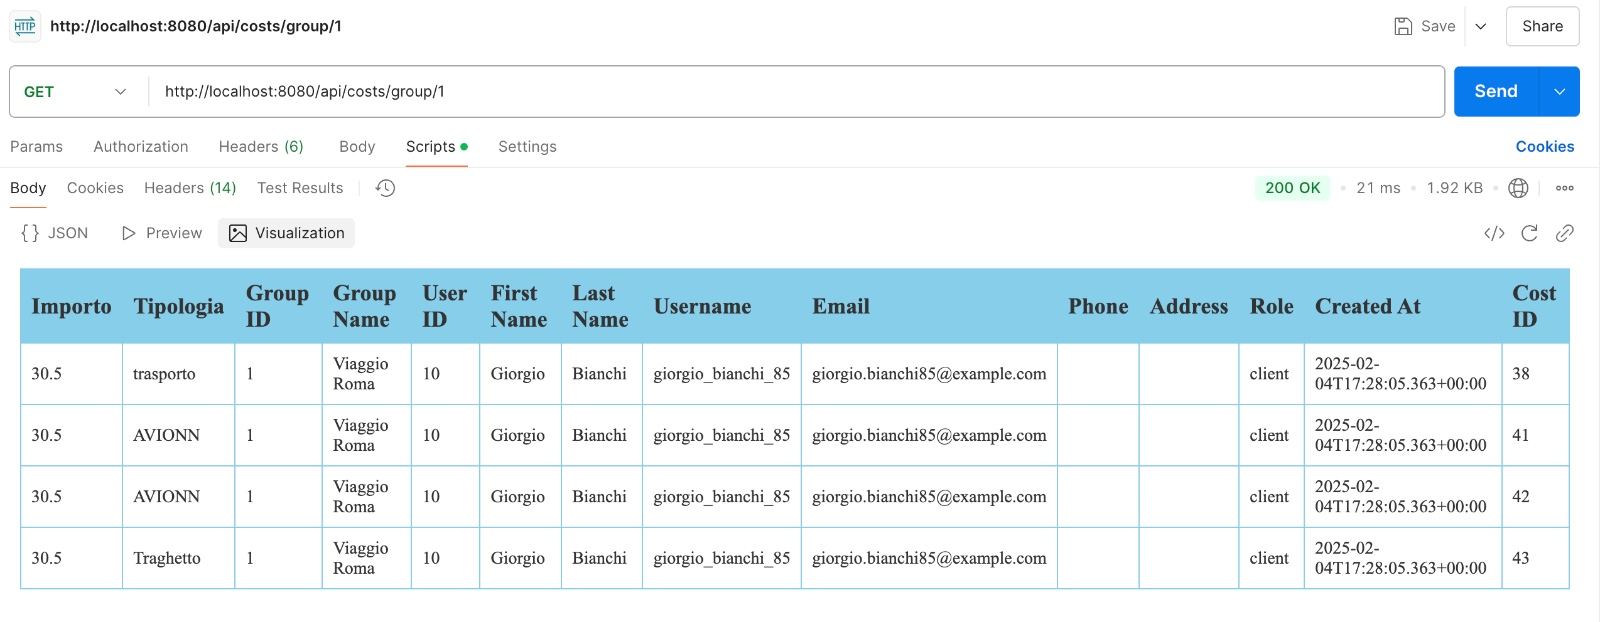
\includegraphics[width=0.9\textwidth]{images/getGroupCosts.jpeg}
    \caption{Risultato API Visualizzazione Costi Gruppo}
    \label{fig:api_view_group_costs}
\end{figure}
